\documentclass[12pt]{article}
\usepackage[utf8]{inputenc}
\usepackage{amsmath, amssymb}
\usepackage{hyperref}
\usepackage{tikz}
\usepackage[left=2.5cm,right=2.5cm,bottom=2.5cm]{geometry}
\usetikzlibrary{arrows, arrows.meta, positioning, bending, quotes}
\hypersetup{
    colorlinks=true}

\title{MATH 5707 (Spring 2026): Homework 7}
\date{}

\begin{document}
\vspace{-0.7in}

\maketitle
\vspace{-0.6in}


\section*{Directions and Introduction}
Submit a pdf of your solutions to the HW 7 assignment on Gradescope by 11:59 pm on April 3.

Problem 3 is marked as a peer review problem. \href{https://docs.google.com/document/d/1jSw9pmMJJFUx_6dTkcUi4k4HJNIrrIIgs9zdWhAycx0/edit?usp=sharing}{This document gives directions and deadlines for the peer review process.}



\section*{Problems}

\begin{enumerate}
\item[0.] If you would like any of these problems to be graded for proficiency with the key skills, list the skill and the corresponding problem.  If you want to label the sill by number, use the numbering that is in the syllabus.
  \item Let $G=(X\sqcup Y,E)$ be a d-regular bipartite multigraph with $d\ge 1$. Show that $|Y|=|E|$. 
    \item Using Kuhn's modified Hungarian Algorithm, find a maximum-weight matching in the graph below. 
   
    \begin{center}
    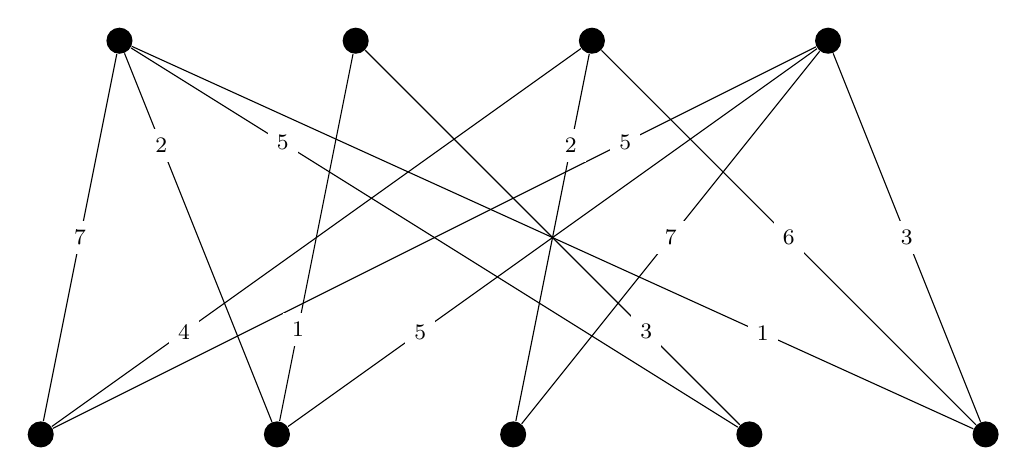
\begin{tikzpicture}
\tikzset{vertex/.style = {shape=circle,fill},every edge quotes/.style={fill=white,font=\footnotesize}}
% vertices
\node[vertex] (a) at  (0,0) {};
\node[vertex] (b) at  (3,0) {};
\node[vertex] (c) at  (6,0) {};
\node[vertex] (d) at  (9,0) {};
\node[vertex] (e) at  (12,0) {};
\node[vertex] (f) at  (1,5) {};
\node[vertex] (g) at  (4,5) {};
\node[vertex] (h) at  (7,5) {};
\node[vertex] (i) at  (10,5) {};

%edges
\path (a) edge["$7$"] (f);

\path (a) edge["$4$" near start] (h);

\path (a) edge["$5$" near end] (i);

\path (b) edge["$2$" near end] (f);

\path (b) edge["$1$"' near start] (g);

\path (b) edge["$5$" near start] (i);

\path (c) edge["$2$" near end] (h);
\path (c) edge["$7$"] (i);
\path (d) edge["$5$" near end] (f);
\path (d) edge["$3$" near start] (g);
\path (e) edge["$6$"] (h);
\path (e) edge["$1$" near start] (f);
\path (e) edge["$3$"] (i);
\end{tikzpicture}

\end{center}  

    \item (Bondy-Murty 5.1.2, peer review problem) Show that every tree has at most one perfect matching.  
  
  \item Give an example of a connected non-Hamiltonian graph that contains two disjoint perfect matchings.  Justify your answer.
  \item Suppose that workers $A$, $B$, $C$, $D$ and $E$ need to do jobs $F$, $G$, $H$, $I$,  and $J$. The table below gives the amount of time that it would take each worker to do each job. Find an assignment where each worker gets one job that minimizes the total time spent on the jobs. (Hint: Turn this scenario into a bipartite graph. By assigning each edge to be the maximum time minus the time for that job, you can translate the problem to be about maximum weight matchings.)
  $$\begin{array}{c|ccccc}
  & A & B & C & D & E\\ \hline
  F & 10 &20 & 13 &8 &15\\
  G & 10 & 15 & 10 & 7 & 12\\
  H & 5 & 8 & 7 & 4 & 9\\
  I & 15 & 20 & 18 & 13 & 15\\
  J & 12 & 15 & 10 & 9 & 13
\end{array}   $$
\end{enumerate}

\end{document}